% Options for packages loaded elsewhere
\PassOptionsToPackage{unicode}{hyperref}
\PassOptionsToPackage{hyphens}{url}
%
\documentclass[
]{article}
\usepackage{lmodern}
\usepackage{amssymb,amsmath}
\usepackage{ifxetex,ifluatex}
\ifnum 0\ifxetex 1\fi\ifluatex 1\fi=0 % if pdftex
  \usepackage[T1]{fontenc}
  \usepackage[utf8]{inputenc}
  \usepackage{textcomp} % provide euro and other symbols
\else % if luatex or xetex
  \usepackage{unicode-math}
  \defaultfontfeatures{Scale=MatchLowercase}
  \defaultfontfeatures[\rmfamily]{Ligatures=TeX,Scale=1}
\fi
% Use upquote if available, for straight quotes in verbatim environments
\IfFileExists{upquote.sty}{\usepackage{upquote}}{}
\IfFileExists{microtype.sty}{% use microtype if available
  \usepackage[]{microtype}
  \UseMicrotypeSet[protrusion]{basicmath} % disable protrusion for tt fonts
}{}
\makeatletter
\@ifundefined{KOMAClassName}{% if non-KOMA class
  \IfFileExists{parskip.sty}{%
    \usepackage{parskip}
  }{% else
    \setlength{\parindent}{0pt}
    \setlength{\parskip}{6pt plus 2pt minus 1pt}}
}{% if KOMA class
  \KOMAoptions{parskip=half}}
\makeatother
\usepackage{xcolor}
\IfFileExists{xurl.sty}{\usepackage{xurl}}{} % add URL line breaks if available
\IfFileExists{bookmark.sty}{\usepackage{bookmark}}{\usepackage{hyperref}}
\hypersetup{
  pdftitle={Homework \#2},
  pdfauthor={David Nemirovsky},
  hidelinks,
  pdfcreator={LaTeX via pandoc}}
\urlstyle{same} % disable monospaced font for URLs
\usepackage[margin=1in]{geometry}
\usepackage{color}
\usepackage{fancyvrb}
\newcommand{\VerbBar}{|}
\newcommand{\VERB}{\Verb[commandchars=\\\{\}]}
\DefineVerbatimEnvironment{Highlighting}{Verbatim}{commandchars=\\\{\}}
% Add ',fontsize=\small' for more characters per line
\usepackage{framed}
\definecolor{shadecolor}{RGB}{248,248,248}
\newenvironment{Shaded}{\begin{snugshade}}{\end{snugshade}}
\newcommand{\AlertTok}[1]{\textcolor[rgb]{0.94,0.16,0.16}{#1}}
\newcommand{\AnnotationTok}[1]{\textcolor[rgb]{0.56,0.35,0.01}{\textbf{\textit{#1}}}}
\newcommand{\AttributeTok}[1]{\textcolor[rgb]{0.77,0.63,0.00}{#1}}
\newcommand{\BaseNTok}[1]{\textcolor[rgb]{0.00,0.00,0.81}{#1}}
\newcommand{\BuiltInTok}[1]{#1}
\newcommand{\CharTok}[1]{\textcolor[rgb]{0.31,0.60,0.02}{#1}}
\newcommand{\CommentTok}[1]{\textcolor[rgb]{0.56,0.35,0.01}{\textit{#1}}}
\newcommand{\CommentVarTok}[1]{\textcolor[rgb]{0.56,0.35,0.01}{\textbf{\textit{#1}}}}
\newcommand{\ConstantTok}[1]{\textcolor[rgb]{0.00,0.00,0.00}{#1}}
\newcommand{\ControlFlowTok}[1]{\textcolor[rgb]{0.13,0.29,0.53}{\textbf{#1}}}
\newcommand{\DataTypeTok}[1]{\textcolor[rgb]{0.13,0.29,0.53}{#1}}
\newcommand{\DecValTok}[1]{\textcolor[rgb]{0.00,0.00,0.81}{#1}}
\newcommand{\DocumentationTok}[1]{\textcolor[rgb]{0.56,0.35,0.01}{\textbf{\textit{#1}}}}
\newcommand{\ErrorTok}[1]{\textcolor[rgb]{0.64,0.00,0.00}{\textbf{#1}}}
\newcommand{\ExtensionTok}[1]{#1}
\newcommand{\FloatTok}[1]{\textcolor[rgb]{0.00,0.00,0.81}{#1}}
\newcommand{\FunctionTok}[1]{\textcolor[rgb]{0.00,0.00,0.00}{#1}}
\newcommand{\ImportTok}[1]{#1}
\newcommand{\InformationTok}[1]{\textcolor[rgb]{0.56,0.35,0.01}{\textbf{\textit{#1}}}}
\newcommand{\KeywordTok}[1]{\textcolor[rgb]{0.13,0.29,0.53}{\textbf{#1}}}
\newcommand{\NormalTok}[1]{#1}
\newcommand{\OperatorTok}[1]{\textcolor[rgb]{0.81,0.36,0.00}{\textbf{#1}}}
\newcommand{\OtherTok}[1]{\textcolor[rgb]{0.56,0.35,0.01}{#1}}
\newcommand{\PreprocessorTok}[1]{\textcolor[rgb]{0.56,0.35,0.01}{\textit{#1}}}
\newcommand{\RegionMarkerTok}[1]{#1}
\newcommand{\SpecialCharTok}[1]{\textcolor[rgb]{0.00,0.00,0.00}{#1}}
\newcommand{\SpecialStringTok}[1]{\textcolor[rgb]{0.31,0.60,0.02}{#1}}
\newcommand{\StringTok}[1]{\textcolor[rgb]{0.31,0.60,0.02}{#1}}
\newcommand{\VariableTok}[1]{\textcolor[rgb]{0.00,0.00,0.00}{#1}}
\newcommand{\VerbatimStringTok}[1]{\textcolor[rgb]{0.31,0.60,0.02}{#1}}
\newcommand{\WarningTok}[1]{\textcolor[rgb]{0.56,0.35,0.01}{\textbf{\textit{#1}}}}
\usepackage{graphicx,grffile}
\makeatletter
\def\maxwidth{\ifdim\Gin@nat@width>\linewidth\linewidth\else\Gin@nat@width\fi}
\def\maxheight{\ifdim\Gin@nat@height>\textheight\textheight\else\Gin@nat@height\fi}
\makeatother
% Scale images if necessary, so that they will not overflow the page
% margins by default, and it is still possible to overwrite the defaults
% using explicit options in \includegraphics[width, height, ...]{}
\setkeys{Gin}{width=\maxwidth,height=\maxheight,keepaspectratio}
% Set default figure placement to htbp
\makeatletter
\def\fps@figure{htbp}
\makeatother
\setlength{\emergencystretch}{3em} % prevent overfull lines
\providecommand{\tightlist}{%
  \setlength{\itemsep}{0pt}\setlength{\parskip}{0pt}}
\setcounter{secnumdepth}{-\maxdimen} % remove section numbering

\title{Homework \#2}
\author{David Nemirovsky}
\date{2/28/21}

\begin{document}
\maketitle

In this exercise, we build nonlinear models using the \College" data.
The dataset contains statistics for 565 US Colleges from the 1995 issue
of US News and World Report. The response variable is the out-of-state
tuition (Outstate). The predictors are:

\begin{itemize}
\item
  Apps: Number of applications received
\item
  Accept: Number of applications accepted
\item
  Enroll: Number of new students enrolled
\item
  Top10perc: Pct. new students from top 10\% of H.S. class
\item
  Top25perc: Pct. new students from top 25\% of H.S. class
\item
  F.Undergrad: Number of fulltime undergraduates
\item
  P.Undergrad: Number of parttime undergraduates
\item
  Room.Board: Room and board costs
\item
  Books: Estimated book costs
\item
  Personal: Estimated personal spending
\item
  PhD: Pct. of faculty with Ph.D.'s
\item
  Terminal: Pct. of faculty with terminal degree
\item
  S.F.Ratio: Student/faculty ratio
\item
  perc.alumni: Pct. alumni who donate
\item
  Expend: Instructional expenditure per student
\item
  Grad.Rate: Graduation rate
\end{itemize}

\hypertarget{a-eda}{%
\subsection{\texorpdfstring{\textbf{a) EDA}}{a) EDA}}\label{a-eda}}

\begin{itemize}
\tightlist
\item
  Read in data and create scatter plots of response (out-of-state
  tuition) vs predictor for each predictor stated above:
\end{itemize}

\begin{Shaded}
\begin{Highlighting}[]
\NormalTok{college_df =}\StringTok{ }
\StringTok{  }\KeywordTok{read_csv}\NormalTok{(}\StringTok{"College.csv"}\NormalTok{) }\OperatorTok\StringTok{ }
\StringTok{  }\NormalTok{janitor}\OperatorTok{::}\KeywordTok{clean_names}\NormalTok{() }\OperatorTok\StringTok{ }
\StringTok{  }\KeywordTok{drop_na}\NormalTok{()}

\NormalTok{x =}\StringTok{ }\KeywordTok{model.matrix}\NormalTok{(outstate }\OperatorTok{~}\StringTok{ }\NormalTok{. }\OperatorTok{-}\NormalTok{college, college_df)[ ,}\OperatorTok{-}\DecValTok{1}\NormalTok{]}
\NormalTok{y =}\StringTok{ }\NormalTok{college_df}\OperatorTok{$}\NormalTok{outstate}

\NormalTok{theme1 =}\StringTok{ }\KeywordTok{trellis.par.get}\NormalTok{()}
\NormalTok{theme1}\OperatorTok{$}\NormalTok{plot.symbol}\OperatorTok{$}\NormalTok{col =}\StringTok{ }\KeywordTok{rgb}\NormalTok{(.}\DecValTok{2}\NormalTok{, }\FloatTok{.4}\NormalTok{, }\FloatTok{.2}\NormalTok{, }\FloatTok{.5}\NormalTok{)}
\NormalTok{theme1}\OperatorTok{$}\NormalTok{plot.symbol}\OperatorTok{$}\NormalTok{pch =}\StringTok{ }\DecValTok{16}
\NormalTok{theme1}\OperatorTok{$}\NormalTok{plot.line}\OperatorTok{$}\NormalTok{col =}\StringTok{ }\KeywordTok{rgb}\NormalTok{(.}\DecValTok{8}\NormalTok{, }\FloatTok{.1}\NormalTok{, }\FloatTok{.1}\NormalTok{, }\DecValTok{1}\NormalTok{)}
\NormalTok{theme1}\OperatorTok{$}\NormalTok{plot.line}\OperatorTok{$}\NormalTok{lwd =}\StringTok{ }\DecValTok{2}
\NormalTok{theme1}\OperatorTok{$}\NormalTok{strip.background}\OperatorTok{$}\NormalTok{col =}\StringTok{ }\KeywordTok{rgb}\NormalTok{(.}\DecValTok{0}\NormalTok{, }\FloatTok{.2}\NormalTok{, }\FloatTok{.6}\NormalTok{, }\FloatTok{.2}\NormalTok{)}
\KeywordTok{trellis.par.set}\NormalTok{(theme1)}
\KeywordTok{featurePlot}\NormalTok{(x, y, }\DataTypeTok{plot =} \StringTok{"scatter"}\NormalTok{, }\DataTypeTok{labels =} \KeywordTok{c}\NormalTok{(}\StringTok{""}\NormalTok{, }\StringTok{"Out of State Tuition"}\NormalTok{), }\DataTypeTok{type =} \KeywordTok{c}\NormalTok{(}\StringTok{"p"}\NormalTok{), }\DataTypeTok{layout =} \KeywordTok{c}\NormalTok{(}\DecValTok{4}\NormalTok{, }\DecValTok{2}\NormalTok{))}
\end{Highlighting}
\end{Shaded}

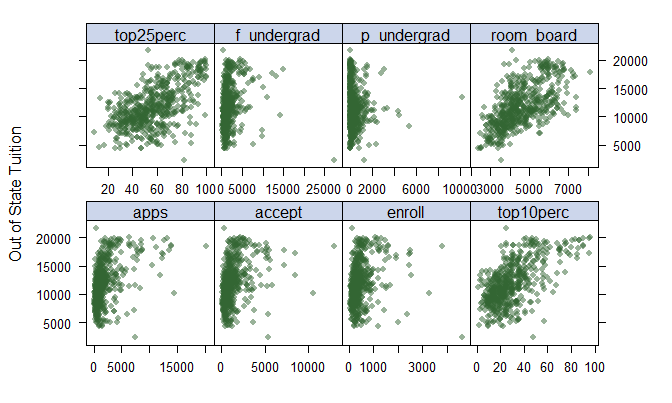
\includegraphics[width=0.95\linewidth]{Homework-2_files/figure-latex/eda-1}
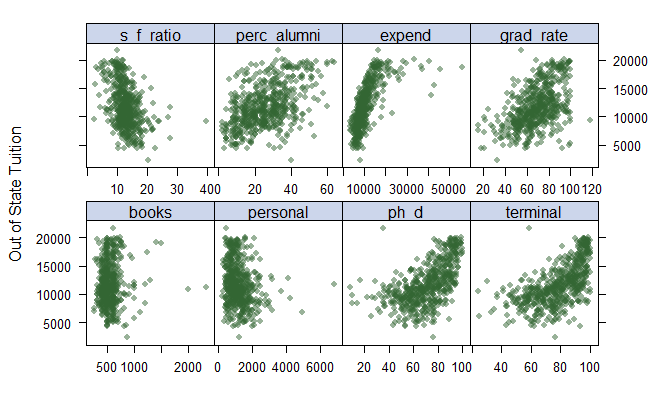
\includegraphics[width=0.95\linewidth]{Homework-2_files/figure-latex/eda-2}

\begin{itemize}
\tightlist
\item
  According to the above plots, percentage of new students from top 25\%
  of H.S. class, percentage of new students from top 10\% of H.S. class,
  room and board costs, student/faculty ratio, percentage of alumni who
  donate, instructional expenditure per student, graduation rate,
  percentage of faculty with Ph.D.'s, and percentage of faculty with
  terminal degrees seem to be the variables that are moderately- to
  highly-correlated with out-of-state tuition. All of the aforementioned
  variables showed a positive correlation with the exception of
  student/faculty ratio.
\end{itemize}

\hypertarget{b-predicting-out-of-state-tuition-using-smoothing-spline-model-of-percentage-of-faculty-with-a-terminal-degree}{%
\subsection{\texorpdfstring{\textbf{b) Predicting Out-of-State Tuition
Using Smoothing Spline Model of Percentage of Faculty with a Terminal
Degree}}{b) Predicting Out-of-State Tuition Using Smoothing Spline Model of Percentage of Faculty with a Terminal Degree}}\label{b-predicting-out-of-state-tuition-using-smoothing-spline-model-of-percentage-of-faculty-with-a-terminal-degree}}

\begin{itemize}
\tightlist
\item
  First, plot smoothing spline models with varying degrees of freedom
  (1-6):
\end{itemize}

\begin{Shaded}
\begin{Highlighting}[]
\NormalTok{term_grid =}\StringTok{ }\KeywordTok{seq}\NormalTok{(}\KeywordTok{range}\NormalTok{(college_df}\OperatorTok{$}\NormalTok{terminal)[}\DecValTok{1}\NormalTok{], }\KeywordTok{range}\NormalTok{(college_df}\OperatorTok{$}\NormalTok{terminal)[}\DecValTok{2}\NormalTok{])}

\NormalTok{ss_df =}\StringTok{ }
\StringTok{  }\KeywordTok{tibble}\NormalTok{(}\DataTypeTok{deg_free =} \DecValTok{1}\OperatorTok{:}\DecValTok{6}\NormalTok{) }\OperatorTok\StringTok{ }
\StringTok{  }\KeywordTok{mutate}\NormalTok{(}
    \DataTypeTok{ss_mod =} \KeywordTok{map}\NormalTok{(}\DataTypeTok{.x =}\NormalTok{ deg_free, }\OperatorTok{~}\KeywordTok{smooth.spline}\NormalTok{(college_df}\OperatorTok{$}\NormalTok{terminal, college_df}\OperatorTok{$}\NormalTok{outstate, }\DataTypeTok{df =}\NormalTok{ .x)), }
    \DataTypeTok{pred =} \KeywordTok{map}\NormalTok{(}\DataTypeTok{.x =}\NormalTok{ ss_mod, }\OperatorTok{~}\KeywordTok{predict}\NormalTok{(.x, }\DataTypeTok{x =}\NormalTok{ term_grid))) }\OperatorTok\StringTok{ }
\StringTok{  }\KeywordTok{select}\NormalTok{(deg_free, pred) }\OperatorTok\StringTok{ }
\StringTok{  }\KeywordTok{unnest}\NormalTok{(pred) }\OperatorTok\StringTok{ }
\StringTok{  }\KeywordTok{unnest}\NormalTok{() }\OperatorTok\StringTok{ }
\StringTok{  }\KeywordTok{filter}\NormalTok{(pred }\OperatorTok{>}\StringTok{ }\DecValTok{100}\NormalTok{) }\OperatorTok\StringTok{ }
\StringTok{  }\KeywordTok{mutate}\NormalTok{(}
    \DataTypeTok{term =} \KeywordTok{c}\NormalTok{(}\KeywordTok{rep}\NormalTok{(term_grid, }\DecValTok{6}\NormalTok{)), }
    \DataTypeTok{deg_free =} \KeywordTok{as.factor}\NormalTok{(deg_free)}
\NormalTok{  )}
\end{Highlighting}
\end{Shaded}

\begin{verbatim}
## Warning: Problem with `mutate()` input `ss_mod`.
## i not using invalid df; must have 1 < df <= n := #{unique x} = 65
## i Input `ss_mod` is `map(...)`.
\end{verbatim}

\begin{verbatim}
## Warning in smooth.spline(college_df$terminal, college_df$outstate, df = .x): not
## using invalid df; must have 1 < df <= n := #{unique x} = 65
\end{verbatim}

\begin{verbatim}
## Warning: `cols` is now required when using unnest().
## Please use `cols = c(pred)`
\end{verbatim}

\begin{Shaded}
\begin{Highlighting}[]
\NormalTok{college_df }\OperatorTok\StringTok{ }
\StringTok{  }\KeywordTok{ggplot}\NormalTok{(}\KeywordTok{aes}\NormalTok{(}\DataTypeTok{x =}\NormalTok{ terminal, }\DataTypeTok{y =}\NormalTok{ outstate)) }\OperatorTok{+}\StringTok{ }
\StringTok{  }\KeywordTok{geom_point}\NormalTok{(}\DataTypeTok{alpha =} \FloatTok{.5}\NormalTok{) }\OperatorTok{+}\StringTok{ }
\StringTok{  }\KeywordTok{geom_line}\NormalTok{(}\KeywordTok{aes}\NormalTok{(}\DataTypeTok{x =}\NormalTok{ term, }\DataTypeTok{y =}\NormalTok{ pred, }\DataTypeTok{color =}\NormalTok{ deg_free), }\DataTypeTok{data =}\NormalTok{ ss_df) }\OperatorTok{+}\StringTok{ }
\StringTok{  }\KeywordTok{labs}\NormalTok{(}\DataTypeTok{title =} \StringTok{"Out-of-State Tuition vs % Faculty with Terminal Degree Smoothing Spline Model by Degrees of Freedom"}\NormalTok{, }
       \DataTypeTok{x =} \StringTok{"Faculty with a Terminal Degree (%)"}\NormalTok{, }
       \DataTypeTok{y =} \StringTok{"Out-of-State Tuition ($)"}\NormalTok{)}
\end{Highlighting}
\end{Shaded}

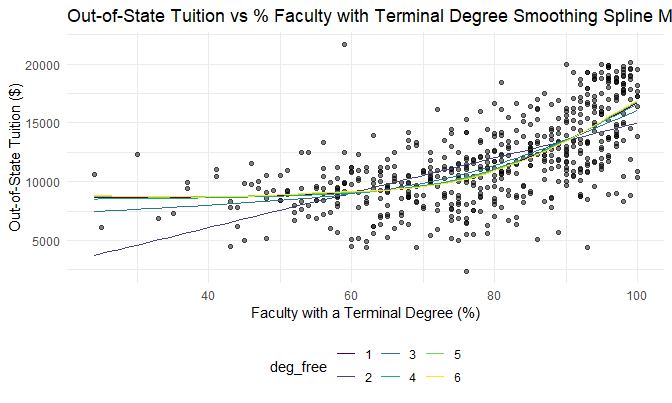
\includegraphics[width=0.95\linewidth]{Homework-2_files/figure-latex/df vary-1}

\begin{itemize}
\item
  Using an arbitrary range of degrees of freedom from 1 to 6, it can be
  seen that an adequate number of degrees of freedom would lie between 4
  and 5, as the lower values (1-3) don't fit the data well and having 6
  degrees of freedom results in a model that is not as smooth.
\item
  Next, use generalized cross-validation (GCV) to select degrees of
  freedom:
\end{itemize}

\begin{Shaded}
\begin{Highlighting}[]
\NormalTok{ss_gcv =}\StringTok{ }\KeywordTok{smooth.spline}\NormalTok{(college_df}\OperatorTok{$}\NormalTok{terminal, college_df}\OperatorTok{$}\NormalTok{outstate)}

\NormalTok{gcv_df =}\StringTok{ }
\StringTok{  }\KeywordTok{tibble}\NormalTok{(}\DataTypeTok{pred =} \KeywordTok{map}\NormalTok{(}\DataTypeTok{.x =}\NormalTok{ term_grid, }\OperatorTok{~}\KeywordTok{predict}\NormalTok{(ss_gcv, .x))) }\OperatorTok\StringTok{ }
\StringTok{  }\KeywordTok{unnest}\NormalTok{(pred) }\OperatorTok\StringTok{ }
\StringTok{  }\KeywordTok{unnest}\NormalTok{() }\OperatorTok\StringTok{ }
\StringTok{  }\KeywordTok{filter}\NormalTok{(pred }\OperatorTok{>}\StringTok{ }\DecValTok{100}\NormalTok{) }\OperatorTok\StringTok{ }
\StringTok{  }\KeywordTok{mutate}\NormalTok{(}\DataTypeTok{term =}\NormalTok{ term_grid)}
\end{Highlighting}
\end{Shaded}

\begin{verbatim}
## Warning: `cols` is now required when using unnest().
## Please use `cols = c(pred)`
\end{verbatim}

\begin{Shaded}
\begin{Highlighting}[]
\NormalTok{college_df }\OperatorTok\StringTok{ }
\StringTok{  }\KeywordTok{ggplot}\NormalTok{(}\KeywordTok{aes}\NormalTok{(}\DataTypeTok{x =}\NormalTok{ terminal, }\DataTypeTok{y =}\NormalTok{ outstate)) }\OperatorTok{+}\StringTok{ }
\StringTok{  }\KeywordTok{geom_point}\NormalTok{(}\DataTypeTok{alpha =} \FloatTok{.5}\NormalTok{) }\OperatorTok{+}\StringTok{ }
\StringTok{  }\KeywordTok{geom_line}\NormalTok{(}\KeywordTok{aes}\NormalTok{(}\DataTypeTok{x =}\NormalTok{ term, }\DataTypeTok{y =}\NormalTok{ pred), }\DataTypeTok{data =}\NormalTok{ gcv_df) }\OperatorTok{+}\StringTok{ }
\StringTok{  }\KeywordTok{labs}\NormalTok{(}\DataTypeTok{title =} \StringTok{"Out-of-State Tuition vs % Faculty with Terminal Degree Smoothing Spline Model Using GCV"}\NormalTok{, }
       \DataTypeTok{x =} \StringTok{"Faculty with a Terminal Degree (%)"}\NormalTok{, }
       \DataTypeTok{y =} \StringTok{"Out-of-State Tuition ($)"}\NormalTok{)}
\end{Highlighting}
\end{Shaded}

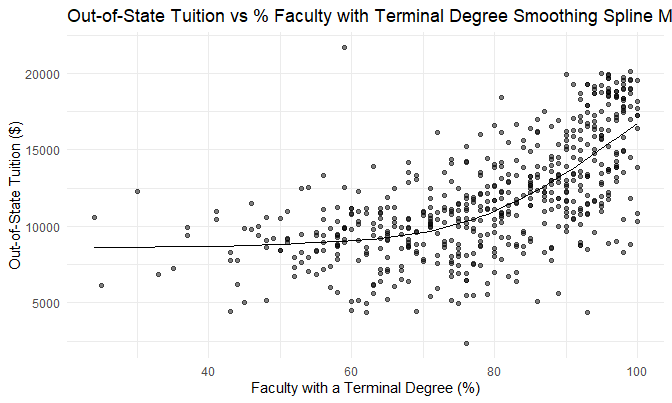
\includegraphics[width=0.95\linewidth]{Homework-2_files/figure-latex/gcv df-1}

\begin{itemize}
\tightlist
\item
  The chosen number of degrees of freedom using GCV is \textbf{4.47}.
  This results in the smoothest model for predicting out-of-stat tuition
  using percentage of faculty with a terminal degree.
\end{itemize}

\hypertarget{c-fitting-a-generalized-additive-model-gam-using-all-predictors}{%
\subsection{\texorpdfstring{\textbf{c) Fitting a Generalized Additive
Model (GAM) Using All
Predictors}}{c) Fitting a Generalized Additive Model (GAM) Using All Predictors}}\label{c-fitting-a-generalized-additive-model-gam-using-all-predictors}}

\begin{itemize}
\tightlist
\item
  Generate GAM models using all predictors:
\end{itemize}

\begin{Shaded}
\begin{Highlighting}[]
\NormalTok{gam_all =}\StringTok{ }\KeywordTok{gam}\NormalTok{(outstate }\OperatorTok{~}\StringTok{ }\NormalTok{apps }\OperatorTok{+}\StringTok{ }\NormalTok{accept }\OperatorTok{+}\StringTok{ }\NormalTok{enroll }\OperatorTok{+}\StringTok{ }\NormalTok{top10perc }\OperatorTok{+}\StringTok{ }\NormalTok{top25perc }\OperatorTok{+}\StringTok{ }\NormalTok{f_undergrad }\OperatorTok{+}\StringTok{ }\NormalTok{p_undergrad }\OperatorTok{+}\StringTok{ }\NormalTok{room_board }\OperatorTok{+}\StringTok{ }\NormalTok{books }\OperatorTok{+}\StringTok{ }\NormalTok{personal }\OperatorTok{+}\StringTok{ }\NormalTok{ph_d }\OperatorTok{+}\StringTok{ }\NormalTok{terminal }\OperatorTok{+}\StringTok{ }\NormalTok{s_f_ratio }\OperatorTok{+}\StringTok{ }\NormalTok{perc_alumni }\OperatorTok{+}\StringTok{ }\NormalTok{expend }\OperatorTok{+}\StringTok{ }\NormalTok{grad_rate, }\DataTypeTok{data =}\NormalTok{ college_df)}

\NormalTok{gam_int =}\StringTok{ }\KeywordTok{gam}\NormalTok{(outstate }\OperatorTok{~}\StringTok{ }\NormalTok{apps }\OperatorTok{+}\StringTok{ }\NormalTok{accept }\OperatorTok{+}\StringTok{ }\NormalTok{enroll }\OperatorTok{+}\StringTok{ }\KeywordTok{te}\NormalTok{(top10perc, top25perc) }\OperatorTok{+}\StringTok{ }\NormalTok{f_undergrad }\OperatorTok{+}\StringTok{ }\NormalTok{p_undergrad }\OperatorTok{+}\StringTok{ }\NormalTok{room_board }\OperatorTok{+}\StringTok{ }\NormalTok{books }\OperatorTok{+}\StringTok{ }\NormalTok{personal }\OperatorTok{+}\StringTok{ }\NormalTok{ph_d }\OperatorTok{+}\StringTok{ }\NormalTok{terminal }\OperatorTok{+}\StringTok{ }\NormalTok{s_f_ratio }\OperatorTok{+}\StringTok{ }\NormalTok{perc_alumni }\OperatorTok{+}\StringTok{ }\NormalTok{expend }\OperatorTok{+}\StringTok{ }\NormalTok{grad_rate, }\DataTypeTok{data =}\NormalTok{ college_df)}

\NormalTok{gam_smooth =}\StringTok{ }\KeywordTok{gam}\NormalTok{(outstate }\OperatorTok{~}\StringTok{ }\NormalTok{apps }\OperatorTok{+}\StringTok{ }\NormalTok{accept }\OperatorTok{+}\StringTok{ }\NormalTok{enroll }\OperatorTok{+}\StringTok{ }\NormalTok{top10perc }\OperatorTok{+}\StringTok{ }\NormalTok{top25perc }\OperatorTok{+}\StringTok{ }\NormalTok{f_undergrad }\OperatorTok{+}\StringTok{ }\NormalTok{p_undergrad }\OperatorTok{+}\StringTok{ }\NormalTok{room_board }\OperatorTok{+}\StringTok{ }\NormalTok{books }\OperatorTok{+}\StringTok{ }\NormalTok{personal }\OperatorTok{+}\StringTok{ }\KeywordTok{s}\NormalTok{(ph_d) }\OperatorTok{+}\StringTok{ }\KeywordTok{s}\NormalTok{(terminal) }\OperatorTok{+}\StringTok{ }\NormalTok{s_f_ratio }\OperatorTok{+}\StringTok{ }\NormalTok{perc_alumni }\OperatorTok{+}\StringTok{ }\NormalTok{expend }\OperatorTok{+}\StringTok{ }\NormalTok{grad_rate, }\DataTypeTok{data =}\NormalTok{ college_df)}

\NormalTok{gam_fin =}\StringTok{ }\NormalTok{gam_inter =}\StringTok{ }\KeywordTok{gam}\NormalTok{(outstate }\OperatorTok{~}\StringTok{ }\NormalTok{apps }\OperatorTok{+}\StringTok{ }\NormalTok{accept }\OperatorTok{+}\StringTok{ }\NormalTok{enroll }\OperatorTok{+}\StringTok{ }\KeywordTok{te}\NormalTok{(top10perc, top25perc) }\OperatorTok{+}\StringTok{ }\NormalTok{f_undergrad }\OperatorTok{+}\StringTok{ }\NormalTok{p_undergrad }\OperatorTok{+}\StringTok{ }\NormalTok{room_board }\OperatorTok{+}\StringTok{ }\NormalTok{books }\OperatorTok{+}\StringTok{ }\NormalTok{personal }\OperatorTok{+}\StringTok{ }\KeywordTok{s}\NormalTok{(ph_d) }\OperatorTok{+}\StringTok{ }\KeywordTok{s}\NormalTok{(terminal) }\OperatorTok{+}\StringTok{ }\NormalTok{s_f_ratio }\OperatorTok{+}\StringTok{ }\NormalTok{perc_alumni }\OperatorTok{+}\StringTok{ }\NormalTok{expend }\OperatorTok{+}\StringTok{ }\NormalTok{grad_rate, }\DataTypeTok{data =}\NormalTok{ college_df)}

\KeywordTok{anova}\NormalTok{(gam_all, gam_int, gam_smooth, gam_fin, }\DataTypeTok{test =} \StringTok{"F"}\NormalTok{)}
\end{Highlighting}
\end{Shaded}

\begin{verbatim}
## Analysis of Deviance Table
## 
## Model 1: outstate ~ apps + accept + enroll + top10perc + top25perc + f_undergrad + 
##     p_undergrad + room_board + books + personal + ph_d + terminal + 
##     s_f_ratio + perc_alumni + expend + grad_rate
## Model 2: outstate ~ apps + accept + enroll + te(top10perc, top25perc) + 
##     f_undergrad + p_undergrad + room_board + books + personal + 
##     ph_d + terminal + s_f_ratio + perc_alumni + expend + grad_rate
## Model 3: outstate ~ apps + accept + enroll + top10perc + top25perc + f_undergrad + 
##     p_undergrad + room_board + books + personal + s(ph_d) + s(terminal) + 
##     s_f_ratio + perc_alumni + expend + grad_rate
## Model 4: outstate ~ apps + accept + enroll + te(top10perc, top25perc) + 
##     f_undergrad + p_undergrad + room_board + books + personal + 
##     s(ph_d) + s(terminal) + s_f_ratio + perc_alumni + expend + 
##     grad_rate
##   Resid. Df Resid. Dev     Df Deviance      F   Pr(>F)   
## 1    547.00 2092185295                                   
## 2    541.70 2027933177 5.2983 64252118 3.3811 0.004270 **
## 3    537.08 1975095132 4.6168 52838045 3.1909 0.009337 **
## 4    532.04 1919385157 5.0410 55709975 3.0812 0.009226 **
## ---
## Signif. codes:  0 '***' 0.001 '**' 0.01 '*' 0.05 '.' 0.1 ' ' 1
\end{verbatim}

\begin{itemize}
\item
  According to the above F-test of the four hypothesized models, the
  model that accounted for the interaction between percentage of new
  students from top 10\% of H.S. class and percentage of new students
  from top 25\% of H.S. class, and the nonparametric variables of
  percentage of faculty with Ph.D.'s and percentage of faculty with
  terminal degrees fit the best GAM. Smoothing splines were used to
  account for the latter two variables.
\item
  Now, plot the GAM:
\end{itemize}

\begin{Shaded}
\begin{Highlighting}[]
\KeywordTok{vis.gam}\NormalTok{(gam_fin, }\DataTypeTok{view =} \KeywordTok{c}\NormalTok{(}\StringTok{"top10perc"}\NormalTok{, }\StringTok{'top25perc'}\NormalTok{), }\DataTypeTok{color =} \StringTok{"topo"}\NormalTok{)}
\end{Highlighting}
\end{Shaded}

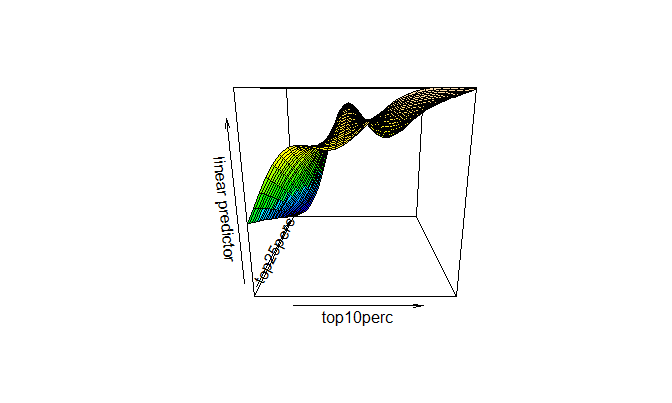
\includegraphics[width=0.95\linewidth]{Homework-2_files/figure-latex/gam plot-1}

\begin{itemize}
\tightlist
\item
  Summary of model:
\end{itemize}

\begin{Shaded}
\begin{Highlighting}[]
\KeywordTok{summary}\NormalTok{(gam_fin)}
\end{Highlighting}
\end{Shaded}

\begin{verbatim}
## 
## Family: gaussian 
## Link function: identity 
## 
## Formula:
## outstate ~ apps + accept + enroll + te(top10perc, top25perc) + 
##     f_undergrad + p_undergrad + room_board + books + personal + 
##     s(ph_d) + s(terminal) + s_f_ratio + perc_alumni + expend + 
##     grad_rate
## 
## Parametric coefficients:
##               Estimate Std. Error t value Pr(>|t|)    
## (Intercept)  4.520e+03  8.319e+02   5.433 8.42e-08 ***
## apps         7.879e-02  1.200e-01   0.657 0.511576    
## accept       1.046e+00  2.170e-01   4.819 1.88e-06 ***
## enroll      -3.264e+00  8.451e-01  -3.862 0.000126 ***
## f_undergrad  2.524e-03  1.320e-01   0.019 0.984750    
## p_undergrad -2.069e-01  1.349e-01  -1.534 0.125550    
## room_board   8.986e-01  9.746e-02   9.221  < 2e-16 ***
## books        9.742e-02  5.107e-01   0.191 0.848785    
## personal    -4.759e-01  1.362e-01  -3.494 0.000515 ***
## s_f_ratio   -2.566e+01  2.843e+01  -0.902 0.367205    
## perc_alumni  4.493e+01  8.353e+00   5.379 1.12e-07 ***
## expend       1.537e-01  2.529e-02   6.078 2.31e-09 ***
## grad_rate    1.878e+01  6.127e+00   3.064 0.002290 ** 
## ---
## Signif. codes:  0 '***' 0.001 '**' 0.01 '*' 0.05 '.' 0.1 ' ' 1
## 
## Approximate significance of smooth terms:
##                           edf Ref.df     F  p-value    
## te(top10perc,top25perc) 6.567  7.520 3.518 0.000825 ***
## s(ph_d)                 4.544  5.612 1.870 0.075698 .  
## s(terminal)             4.745  5.824 1.872 0.079249 .  
## ---
## Signif. codes:  0 '***' 0.001 '**' 0.01 '*' 0.05 '.' 0.1 ' ' 1
## 
## R-sq.(adj) =  0.738   Deviance explained = 75.1%
## GCV = 3.7801e+06  Scale est. = 3.5867e+06  n = 564
\end{verbatim}

\begin{itemize}
\tightlist
\item
  \textbf{According to the final GAM at the 10\% significance level,
  number of applications accepted, number of applications enrolled, room
  and board costs, estimated personal spending, percentage of alumni who
  donate, instructional expenditure per student, graduation rate,
  percentage of new students from top 25\% of H.S. class, percentage of
  new students from top 10\% of H.S. class, and the smoothing splines of
  percentage of faculty with Ph.D.'s and percentage of faculty with
  terminal degrees were all found to be significant predictors of
  out-of-state tuition.}
\end{itemize}

\hypertarget{d-fit-a-multivariate-adaptive-regression-spline-mars-model-using-all-predictors}{%
\subsection{\texorpdfstring{\textbf{d) Fit a Multivariate Adaptive
Regression Spline (MARS) Model Using All
Predictors}}{d) Fit a Multivariate Adaptive Regression Spline (MARS) Model Using All Predictors}}\label{d-fit-a-multivariate-adaptive-regression-spline-mars-model-using-all-predictors}}

\begin{itemize}
\tightlist
\item
  First, fit MARS models to determine best one:
\end{itemize}

\begin{Shaded}
\begin{Highlighting}[]
\NormalTok{mars_grid =}\StringTok{ }\KeywordTok{expand.grid}\NormalTok{(}\DataTypeTok{degree =} \DecValTok{1}\OperatorTok{:}\DecValTok{3}\NormalTok{, }
                         \DataTypeTok{nprune =} \DecValTok{2}\OperatorTok{:}\DecValTok{18}\NormalTok{)}
\NormalTok{ctrl =}\StringTok{ }\KeywordTok{trainControl}\NormalTok{(}\DataTypeTok{method =} \StringTok{"cv"}\NormalTok{, }\DataTypeTok{number =} \DecValTok{10}\NormalTok{)}
\KeywordTok{set.seed}\NormalTok{(}\DecValTok{37564}\NormalTok{)}

\NormalTok{mars_fit <-}\StringTok{ }\KeywordTok{train}\NormalTok{(x, y,}
                  \DataTypeTok{method =} \StringTok{"earth"}\NormalTok{,}
                  \DataTypeTok{tuneGrid =}\NormalTok{ mars_grid,}
                  \DataTypeTok{trControl =}\NormalTok{ ctrl)}

\KeywordTok{ggplot}\NormalTok{(mars_fit)}
\end{Highlighting}
\end{Shaded}

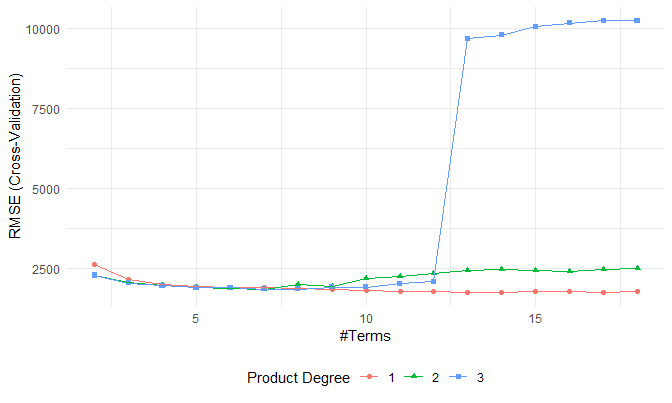
\includegraphics[width=0.95\linewidth]{Homework-2_files/figure-latex/mars mods-1}

\begin{Shaded}
\begin{Highlighting}[]
\NormalTok{mars_fit}\OperatorTok{$}\NormalTok{bestTune}
\end{Highlighting}
\end{Shaded}

\begin{verbatim}
##    nprune degree
## 12     13      1
\end{verbatim}

\begin{Shaded}
\begin{Highlighting}[]
\KeywordTok{coef}\NormalTok{(mars_fit}\OperatorTok{$}\NormalTok{finalModel)}
\end{Highlighting}
\end{Shaded}

\begin{verbatim}
##         (Intercept)     h(expend-15365)  h(4450-room_board)     h(grad_rate-97) 
##       11099.4030981          -0.7308623          -1.2860756        -205.1619640 
##     h(97-grad_rate) h(f_undergrad-1355) h(1355-f_undergrad)   h(22-perc_alumni) 
##         -24.3424023          -0.3435602          -1.3670697         -77.4621692 
##        h(apps-3712)    h(1300-personal)       h(913-enroll)      h(2193-accept) 
##           0.4247957           0.9815494           4.6968931          -2.0136737 
##      h(expend-6881) 
##           0.7344018
\end{verbatim}

\begin{itemize}
\item
  According to the above RMSE plot with varying degrees and number of
  terms, it appears as though the MARS model with \textbf{13} retained
  terms using \textbf{1} degree of interactions generated the lowest
  RMSE, indicating that these tuning parameters fit the best model,
  using all of the variable to predict out-of-state tuition.
\item
  Now, let's examine the partial dependence plot using the percentage of
  alumni who donate as an arbitrary predictor:
\end{itemize}

\begin{Shaded}
\begin{Highlighting}[]
\NormalTok{pdp}\OperatorTok{::}\KeywordTok{partial}\NormalTok{(mars_fit, }\DataTypeTok{pred.var =} \KeywordTok{c}\NormalTok{(}\StringTok{"perc_alumni"}\NormalTok{), }\DataTypeTok{grid.resolution =} \DecValTok{10}\NormalTok{) }\OperatorTok\StringTok{ }\KeywordTok{autoplot}\NormalTok{()}
\end{Highlighting}
\end{Shaded}

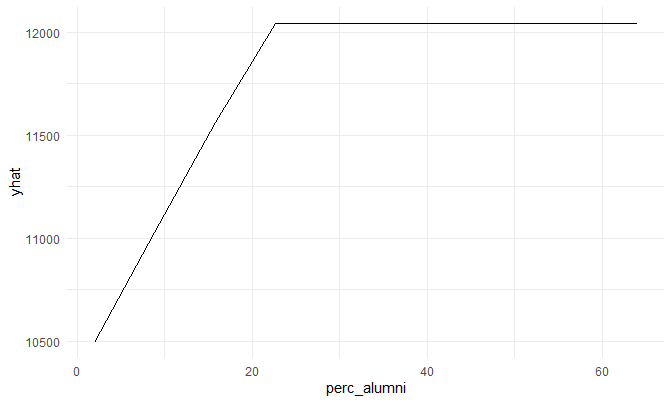
\includegraphics[width=0.95\linewidth]{Homework-2_files/figure-latex/pdp-1}

\begin{itemize}
\tightlist
\item
  The above partial dependence plot of percentage of alumni who donate
  as a predictor for out-of-state tuition shows that percentage of
  alumni who donate does not have as strong of an effect on out-of-state
  tuition after the threshold of \textasciitilde22\%.
\end{itemize}

\end{document}
